\documentclass{beamer}
\mode<presentation>
{
  \usetheme{default}      % or try Darmstadt, Madrid, Warsaw, ...
  \usecolortheme{default} % or try albatross, beaver, crane, ...
  \usefonttheme{default}  % or try serif, structurebold, ...
  \setbeamertemplate{navigation symbols}{}
  \setbeamertemplate{caption}[numbered]
} 


\usepackage[utf8]{inputenc}
\usepackage{default}
\usepackage{listings}

\usepackage{graphicx}
\begin{document}

\section{Introduction}

\subsection{Summary}

\begin{frame}{Owl Summary}
\begin{block} {Highlights}
 \begin{itemize}
  \item A new, self described \textit{Numpy styled} numerical library for OCaml \newline
  \item Designed to be interactive and repl friendly\newline
  \item Backed by gsl and plplot\newline
\end{itemize}
\end{block}
\pause
\begin{block}{\emph{TLDR;}}
\begin{itemize}
  \item Analyze data with sane interfaces 
  \item Make pretty plots with little hassle
 \end{itemize}
\end{block}
\end{frame}


\subsection{About author}

\begin{frame}{About the author - Liang Wang}
\begin{center}
 
\includegraphics[height=45px, width=35px, bb=14 14 120 150]{./liang_wang_smaller.eps}
 % liang_wang_smaller.eps: 0x0 pixel, 300dpi, 0.00x0.00 cm, bb=14 14 120 159
\end{center}

\begin{block}{Credentials}
\begin{itemize}
\item M.Sc and Ph.D degrees from University of Helsinki, Finland
\item Research Associate at Computer Laboratory, Cambridge University
\item Postdoc Research Associate in Queens' College
\end{itemize}
\end{block}
\pause

\begin{block}{In his own words}
\begin{quotation}
My work focuses on information-centric networking, network architecture, network optimisation and protocol design. 
I have strong interest in data analytics and big data framework. I also teach, I am an Associated Fellow in the British Higher Education Academy.
\end{quotation}
\end{block}
\end{frame}

\subsection{Owl vs...}

\begin{frame}{Owl vs Gsl}
\begin{block}{Differences}
\begin{itemize}
 \item developed over a decade ago by Markus Mottl (NYC) 
 \item bindings to Gnu Scientific Library (C, but portable)
 \item makes no attempt to simplify somewhat opaque GSL interfaces
 \item sometimes used as middleware for other math libs (owl, pareto, gpr, libsvm)
\end{itemize}
\end{block}
\end{frame}

\begin{frame}{Owl vs Oml}
\begin{block}{\textbf{(Besides the upside-down w)}}

\end{block}
\begin{block}{Differences}
\begin{itemize}
 \item developed mostly by Leonid Rozenberg of Hammerlab (NYC) in 2015-16 
 \item does not depend on gsl (instead- lacaml,lbfgs,ocepheps)
 \item no built in plotting
 \item provides general math utils but centers around machine learning
 \item usable in repl but not (yet) as convenient for typical data
\end{itemize}
\end{block}
\end{frame}

\begin{frame}{Owl vs Pareto}
\begin{block}{Differences}
\begin{itemize}
\item Authored by Sergei Lebedev in 2013
\item Depends on gsl
\item Focuses primarily on statistics
\item Provides common statistical tests for significant differences between samples.
\item Makes uniform interfaces for common discrete and continuous probability distributions.
\item Features sample statistics, quantile estimation, kernel density estimation.
\end{itemize}
\end{block}
\end{frame}

\begin{frame}{Ocaml And Data Science}
\begin{block}{Leading data science languages}
\begin{itemize}
\item Python - untyped by design
\item R - awkward type system, not a general purpose language
\item Matlab - proprietary, types weak or nonexistant
\item Java and C\# - verbose, type systems inferior to ML / Haskell
\item Scala - still too verbose, suffers from some Java hangups
\item F\# - an interesting choice, if you can tolerate MS ecosystem
\item Julia - gaining momentum, something to watch out for
\end{itemize}
\end{block}
\pause

\begin{block}{Why not...}
\begin{itemize}
\item \textbf{OCaml - perfect choice but needs more data science tooling!}
\pause
\item \textbf {OCaml should be gunning for data scientists!}
\end{itemize}
\end{block}
\end{frame}

\begin{frame}{A quick example}
\lstinputlisting[basicstyle=\tiny, language=ML]{quick-example.ml}
\pause
\begin{center}
 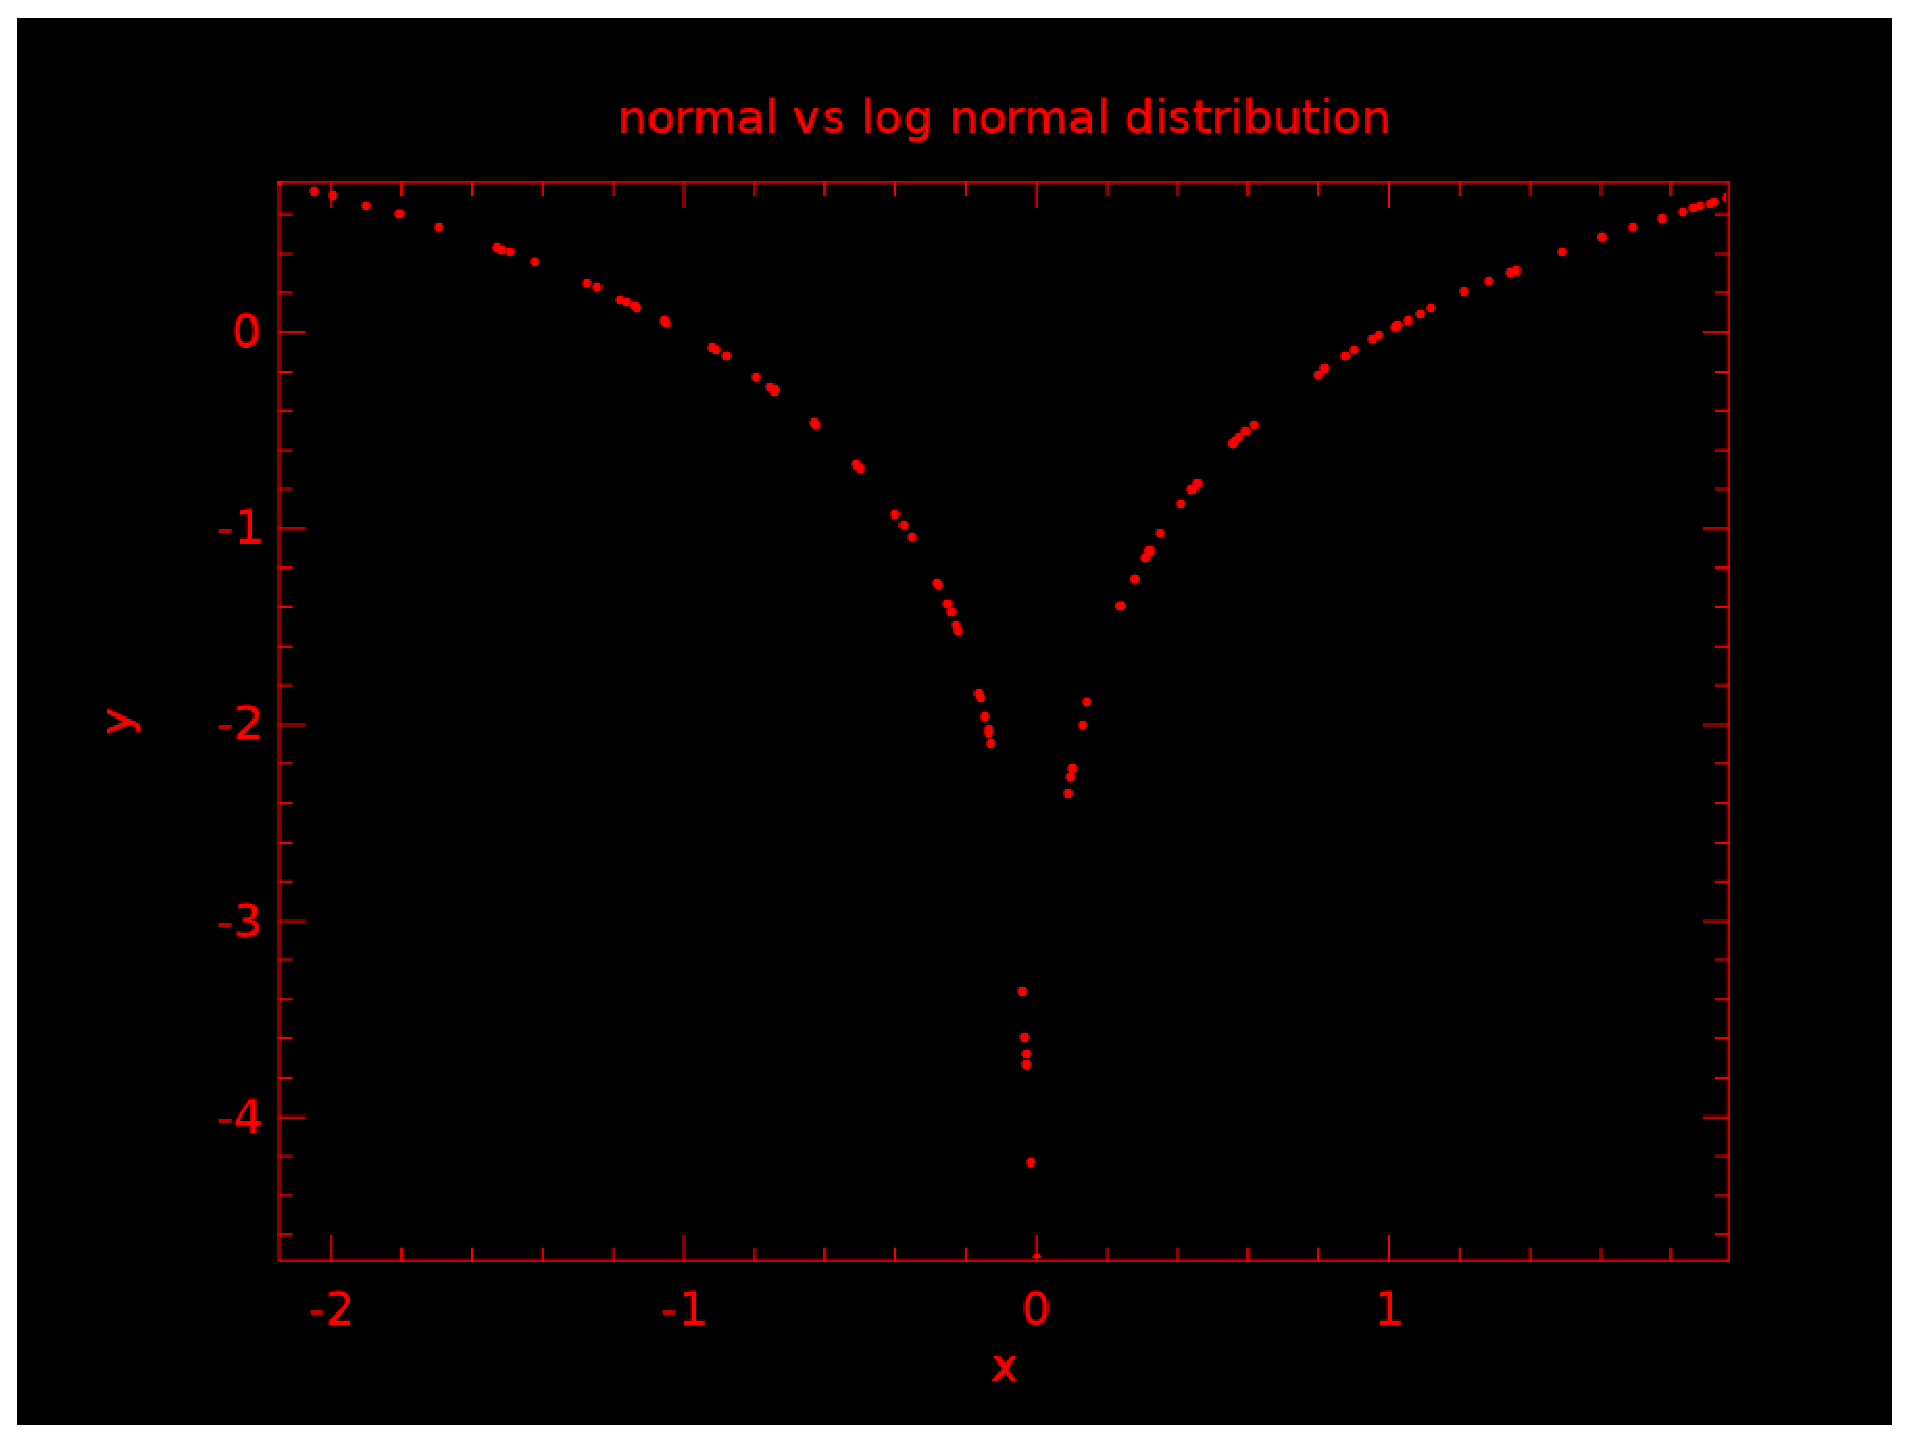
\includegraphics[width=200px,height=150px,bb=14 14 915 690]{./norm-vs-log.eps}
 % norm-vs-log.eps: 0x0 pixel, 300dpi, 0.00x0.00 cm, bb=14 14 915 690
\end{center}
\end{frame}

  \section{Module walkthrough}

\begin{frame}{Modules (Types, Matrices, and Utils)} 
\begin{itemize}
\item \textbf{Owl\_types} -  Define the types shared by various modules
\item \textbf{Owl\_utils} - Helper functions used in the library
 \item \textbf{Owl\_const} - This module is extended from gsl-ocaml by including SI system.
\item \textbf{Owl\_dense} - Dense matrix module
\item \textbf{Owl\_dense\_complex} - Complex dense matrix module: this module supports operations on dense matrices of complex numbers.
\item \textbf{Owl\_dense\_real} - Real dense matrix module
\item \textbf{Owl\_sparse} - Sparse matrix module
\item \textbf{Owl\_sparse\_complex} - Complex sparse matrix: this module supports the operations on sparse matrices of complex numbers.
\item \textbf{Owl\_sparse\_real} - Sparse real matrix: this module supports the operations on sparse matrices of real numbers.
\end{itemize}
\end{frame}

\begin{frame}{Modules (Functions and plotting)}
\begin{itemize}
\item \textbf{Owl\_fft} - Fast Fourier Transforms (FFTs) : this module implements some basic FFT operations.
\item \textbf{Owl\_linalg} - Linear Algebra module
\item \textbf{Owl\_maths} - Mathematics module
\item \textbf{Owl\_optimise} - Machine learning library Note: C layout row-major matrix
\item \textbf{Owl\_plot} - Plot module The input to a plot function is supposed to be a row-based matrix.
\item \textbf{Owl\_pretty} - Generic matrix printing functions.
\item \textbf{Owl\_regression} - Regression module
\item \textbf{Owl\_stats} - Statistics module
\item \textbf{Owl\_toplevel} - Install Toplevel Printers
\end{itemize}
\end{frame}



\begin{frame}{Live plotting in utop}
\textbf{Now let's try to use this thing in real time...}
\end{frame}
\begin{frame}{Acknowledgements and References}

\begin{block}{Special thanks}
\begin{itemize}
\item Jane Street - for the space and OCaml community support!
\item Liang Wang - for writing Owl
\item Markus Mottl - for writing gsl
\end{itemize}
\end{block}
\begin{block}{References}
\begin{itemize}
\item Owl on github: https://github.com/ryanrhymes/owl
\item Owl plotting tutorial: https://github.com/ryanrhymes/owl/wiki/Tutorial:-How-to-Plot-in-Owl?
\item Owl API: http://www.cl.cam.ac.uk/~lw525/owl/
\item gsl-ocaml on github: https://github.com/mmottl/gsl-ocaml
\item Oml on github: https://github.com/hammerlab/oml
\item Pareto on github: https://github.com/superbobry/pareto
\end{itemize}
\end{block}
\end{frame}
\end{document}
